\section{Test Report}

\setlist[enumerate]{itemsep=2pt, topsep=4pt, parsep=0pt}

\subsection{What has been tested}
% Identify items tested (Unit, System, UAT).
% Discuss integration testing if applicable.
% Identify Test Oracles.

The testing strategy for the SPIO Competitor Benchmarking system is structured across four levels: unit testing, integration testing, system testing, and user acceptance testing (UAT). This layered approach ensures that the system is validated both in isolation and as a complete end-to-end platform. Integration testing was treated as a distinct stage because the system’s three-tier architecture, consisting of a React frontend, an Express backend, and a PostgreSQL database, must operate reliably across multiple interacting layers. In addition, the scraping engine contains more than twenty university-specific adapters, making it essential to verify not only the correctness of individual components, but also the robustness of their interactions under realistic conditions.

\begin{figure}[h!]
    \centering
    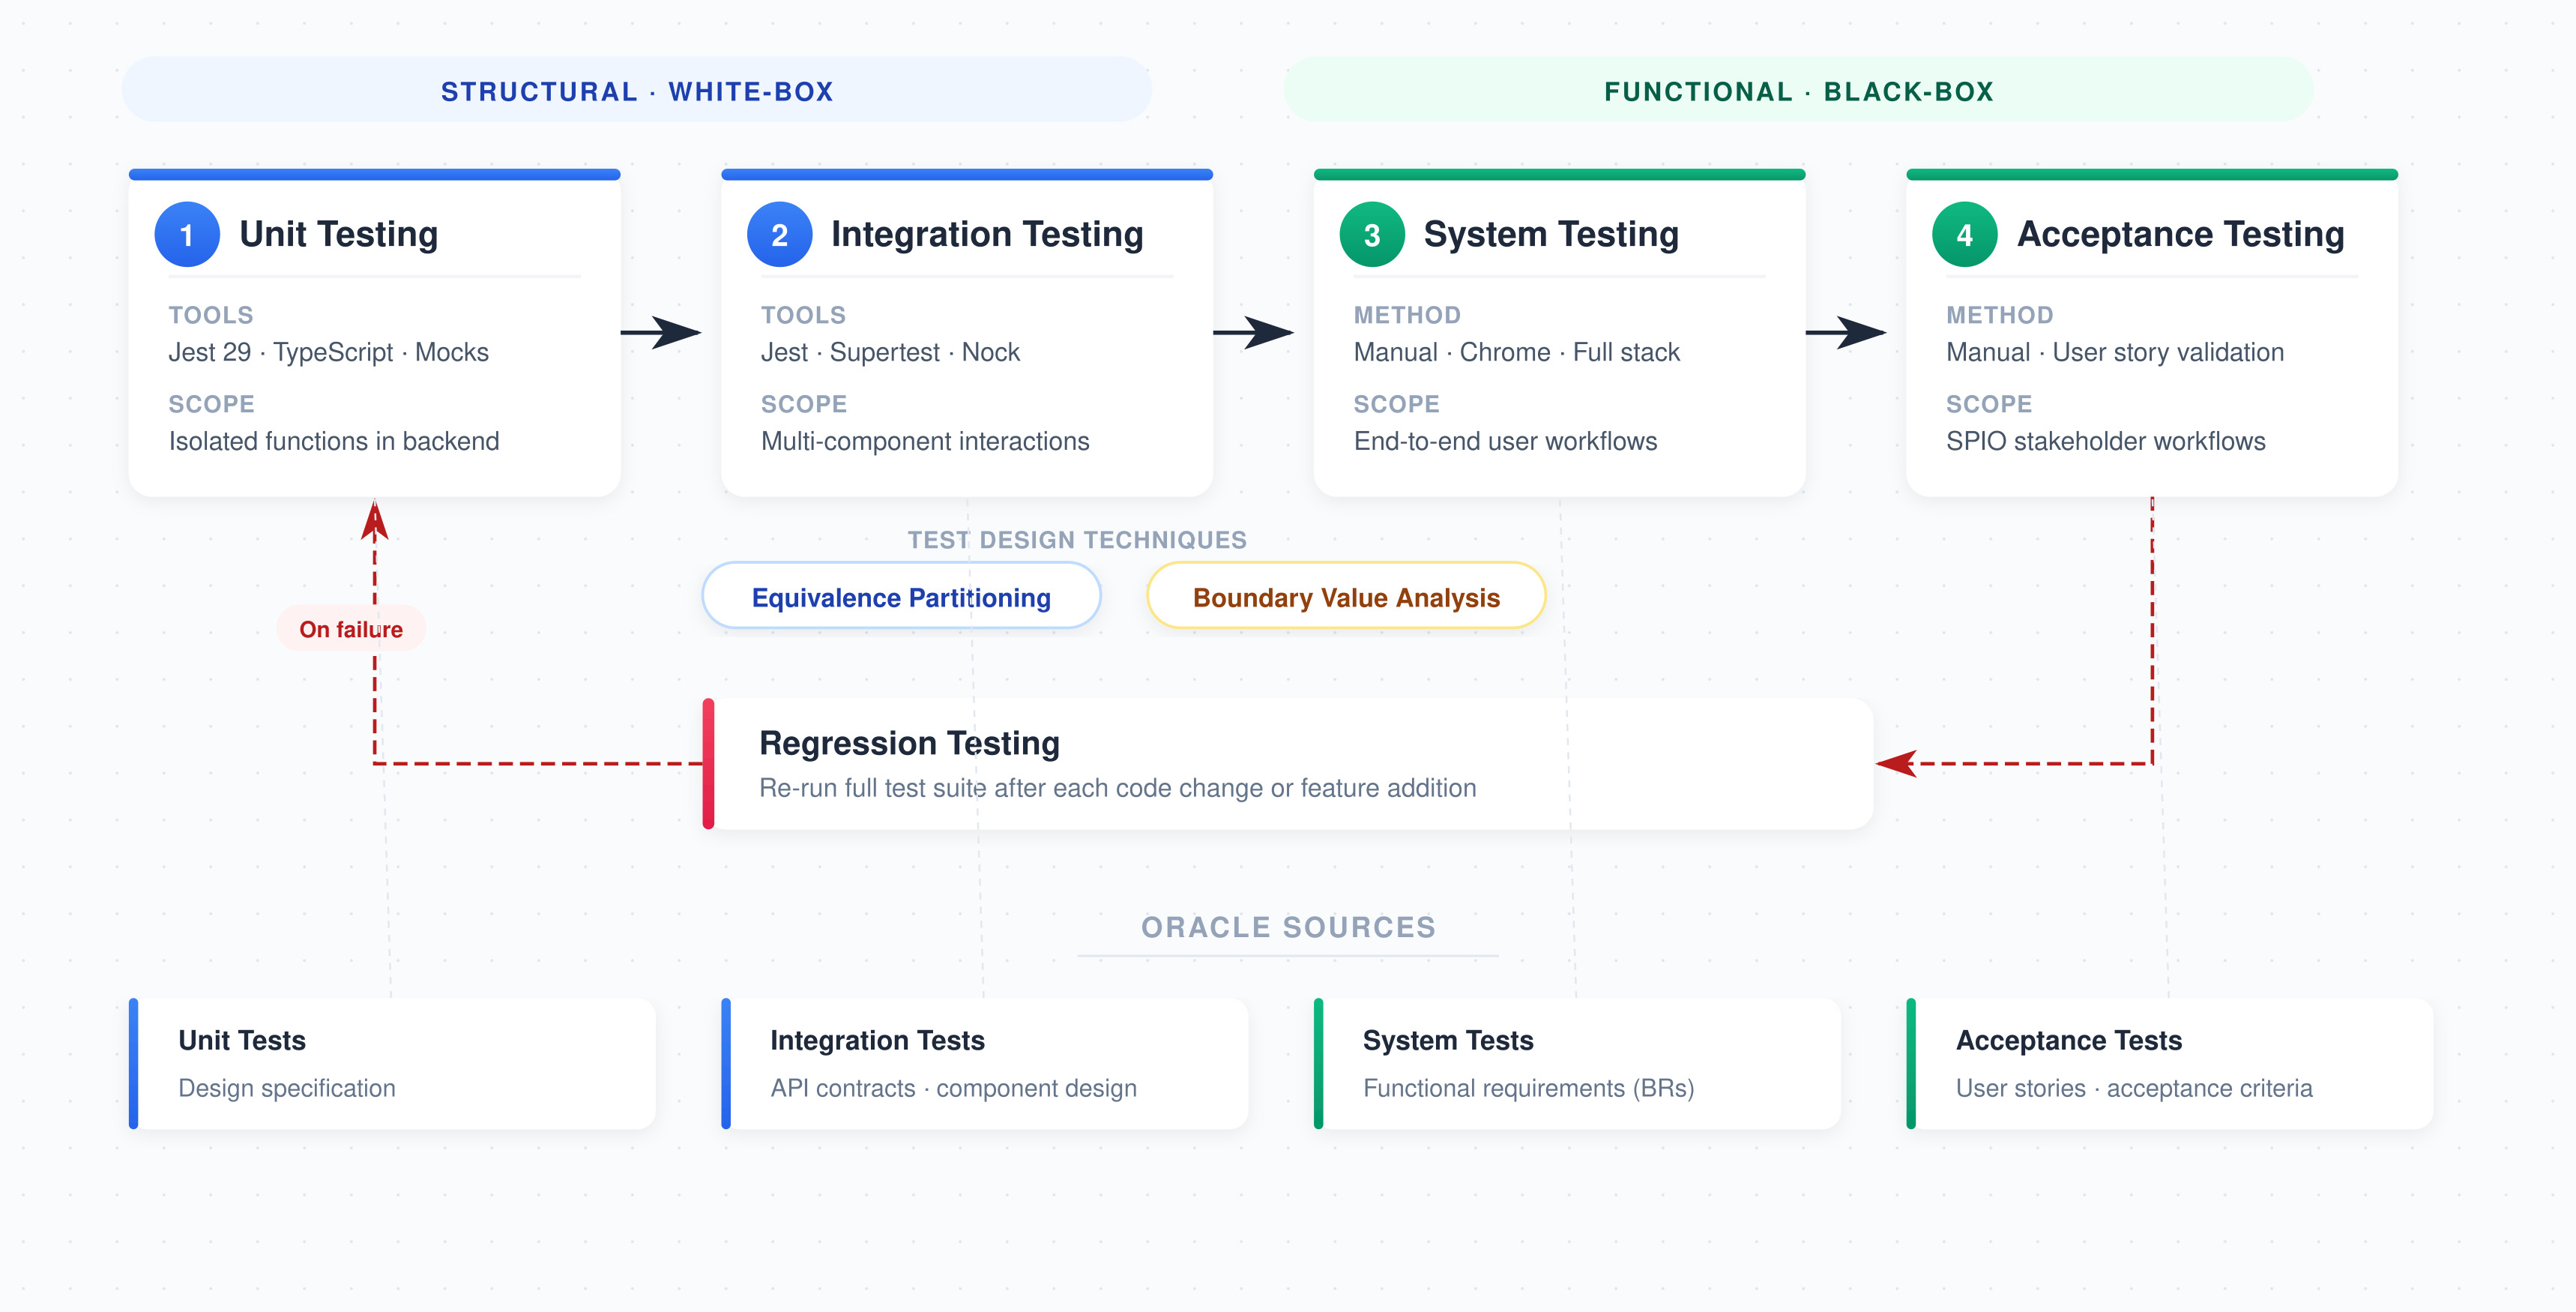
\includegraphics[width=0.85\textwidth]{testing_pipeline_v3.jpg}
    \caption{Overview of the testing pipeline}
    \label{fig:testing-pipeline}
\end{figure}

\subsubsection*{Unit Testing Scope}

Unit tests target isolated backend functions with no database or network access. The following items were tested:

\begin{enumerate}
    \item \textbf{A-Level grade extraction logic} (\texttt{extractALevels} in \texttt{services.ts}) --- parses UCAS qualification data to extract individual A-Level grades from offer strings.
    \item \textbf{Fee histogram binning logic} (from the \texttt{/dashboard/fees} route in \texttt{dashboard.ts}) --- assigns tuition fee values to predefined bins for dashboard bar chart visualisation.
    \item \textbf{Course level classification} (\texttt{determineLevel} in \texttt{visualisation.ts}) --- classifies courses as Undergraduate, Postgraduate, or Other based on outcome qualification strings.
    \item \textbf{Scraper configuration lookup with fuzzy matching} (\texttt{getConfigForUniversity} in \texttt{manager.ts}) --- resolves university names from the UCAS database to internal scraper configurations using exact and substring matching.
\end{enumerate}

\noindent\textbf{Test Oracle:} Expected outputs are derived from the design specification --- specifically, the function signatures, internal data structures, and the known UCAS API format. The oracle type is \textit{example/golden result}: known correct outputs for given inputs.

\subsubsection*{Integration Testing Scope}

Integration tests verify interactions between multiple components working together across the backend stack. The following items were tested:

\begin{enumerate}
    \item \textbf{Full authentication lifecycle} --- the login route (\texttt{auth.ts}), session middleware (\texttt{express-session}), and the \texttt{/auth/me} endpoint operating together to create, persist, and destroy user sessions.
    \item \textbf{Scraper pipeline execution} --- the scraping adapter, manager script, and database writes operating end-to-end with mocked HTTP responses.
    \item \textbf{Courses API with nested database queries} --- the \texttt{/courses} endpoint constructing Prisma queries with multiple filters (university, year, fee range, level) and returning paginated results.
    \item \textbf{Visualisation API data aggregation} --- the \texttt{/visualisation/price-history} endpoint aggregating multi-year tuition fee data via Prisma \texttt{groupBy} and returning the JSON structure consumed by the frontend charts.
\end{enumerate}

\noindent\textbf{Test Oracle:} Expected outputs are derived from the system component design --- the API contracts, database schema, and the expected JSON response structures.

\subsubsection*{System Testing Scope}

System tests validate complete end-to-end user workflows through the full stack (browser $\rightarrow$ frontend $\rightarrow$ backend $\rightarrow$ database). The following items were tested:

\begin{enumerate}
    \item \textbf{Scrape initiation and concurrency locking} --- verifies that only one scraping process can run at a time and that concurrent requests are rejected.
    \item \textbf{Combined search and multi-institution filtering} --- verifies that keyword search and institution filters work together to return the correct subset of courses.
    \item \textbf{Cross-page comparison state persistence} --- verifies that course selections made across paginated pages are retained when navigating to the comparison view.
    \item \textbf{Dataset export with edge case handling} --- verifies that Excel export functions correctly for large datasets and that the export button is disabled when no courses are selected.
\end{enumerate}

\noindent\textbf{Test Oracle:} Expected results are derived from the functional requirements specification --- specifically the behavioural requirements (BR codes) defined in the requirements documentation.

\subsubsection*{User Acceptance Testing Scope}

User acceptance tests verify the system's acceptability from the end-user (SPIO staff) perspective. The following items were tested:

\begin{enumerate}
    \item \textbf{Quick Scrape dashboard workflow} --- the complete scrape initiation, status monitoring, and data refresh cycle from the Dashboard page.
    \item \textbf{Course data export to Excel} --- selecting courses and downloading an Excel file with correct content.
    \item \textbf{Keyword search functionality} --- searching for courses by full name, partial keyword, and non-matching terms.
    \item \textbf{Course comparison and visualisation interaction} --- searching for courses, adding them to the comparison view, removing selections, and navigating to course detail pages.
\end{enumerate}

\noindent\textbf{Test Oracle:} Expected behaviour is derived directly from the user stories and acceptance criteria defined during the requirements phase. This is a \textit{requirements-based} oracle.

\subsubsection*{Test Design Techniques}

Equivalence partitioning (EP) and boundary value analysis (BVA) formed the core of the test design strategy across all testing levels. Equivalence partitioning was used to separate input domains into valid and invalid classes, enabling broad and representative coverage without resorting to exhaustive testing. Boundary value analysis was applied to numeric and range-based inputs, particularly within the fee histogram binning logic, where boundary conditions presented the greatest likelihood of off-by-one defects. Testing effort was further prioritised using defect clustering. Particular emphasis was placed on the scraping engine and authentication modules because these components combined high implementation complexity with heightened operational risk. The scraping engine depended on external data sources, while the authentication module was responsible for security-sensitive behaviour.

\subsection{Test Cases}

% SAMPLE TABLE LAYOUT

% {
% \small
% \renewcommand{\arraystretch}{0.9}
% \begin{xltabular}{\linewidth}{@{} >{\bfseries\raggedright}p{0.22\textwidth} >{\raggedright\arraybackslash}X @{}}
% \toprule
% \multicolumn{2}{@{}l}{\large\bfseries\color{customtitles} int\_test-02 \hfill {\normalsize\color{black!60} Severity: Critical}} \\
% \midrule
% Description          & Backend HTML Scraper Pipeline Execution with Mocked Data \\*[2pt]
% Testing Technique    & Equivalence Partitioning (EP) \\*[2pt]
% Related Req.         & $<$BR 2.1$>$ (Data scraping and storage) \\*[2pt]
% Pre-requisites       & Database contains a single mocked course entry (belonging to Lancaster University) with two course options (full time and part time) that have null fees. Nock is configured to intercept HTTP requests from Axios and return mocked HTML. \\*[2pt]
% Equivalence Classes  & \textbf{EC1} (valid): Both full time and part time fees present in HTML. \newline \textbf{EC2} (valid): Only one fee type is present in HTML. \newline \textbf{EC3} (invalid): No fees present in HTML. \\
% \midrule
% Test Procedure       & \\*[2pt]
% \quad\normalfont\textit{EC1}  & Configure Nock to return \textbf{MO1} \\*[2pt]
% \quad\normalfont\textit{EC2}  & Configure Nock to return \textbf{MO2} \\*[2pt]
% \quad\normalfont\textit{EC3}  & Configure Nock to return \textbf{MO3} \newline Run the scraping manager directly via \texttt{npx ts-node} \\*[2pt]
% Expected Result      & The manager invokes the adapter for Lancaster University, processes the mocked HTML file without timing out, and updates the database where: \newline \textbf{EC1}: The full time course option has \texttt{homeFee: 14140; intlFee: 30000} and the part time course option has \texttt{homeFee: 7070; intlFee: 15000}. \newline \textbf{EC2}: The full time course option has \texttt{homeFee: 14140; intlFee: 30000} and the part time course option has \texttt{homeFee: null; intlFee: null}. \newline \textbf{EC3}: The full time course option has \texttt{homeFee: null; intlFee: null} and the part time course option has \texttt{homeFee: null; intlFee: null}. \\
% \midrule
% Test Material        & 3 mocked HTML files: \textbf{MO1} (both fees present), \textbf{MO2} (only full time fees present), and \textbf{MO3} (no fees present), corresponding to the respectively numbered equivalence classes; 1 mocked database course entry \\*[2pt]
% Comments             & This test validates the core logic behind data extraction and storage, evaluating the performance of scraping adapters and their integration with the database via the manager script. \\*[2pt]
% Created by           & Sam \\*[2pt]
% Test Environment     & Node.js 20, Nock 14, Windows 10 \\
% \bottomrule
% \end{xltabular}
% }



\subsubsection{Unit Testing}

{
\small
\renewcommand{\arraystretch}{0.9}
\begin{xltabular}{\linewidth}{@{} >{\bfseries\raggedright}p{0.22\textwidth} >{\raggedright\arraybackslash}X @{}}
\toprule
\multicolumn{2}{@{}l}{\large\bfseries\color{customtitles} unit\_test-01 -- \color{ForestGreen} PASSED \hfill {\normalsize\color{black!60} Severity: High}} \\
\midrule
Description          & A-Level grade extraction from UCAS qualification data \\*[2pt]
Testing Technique    & Equivalence Partitioning (EP) \\*[2pt]
Related Req.         & $<$BR 2.1$>$ (Data scraping and storage) \\*[2pt]
Pre-requisites       & The \texttt{extractALevels()} function in \texttt{services.ts} is available for isolated invocation with mock data. No database or network access required. \\*[2pt]
Equivalence Classes  & \textbf{EC1} (valid): Standard grade string (e.g.\ ``A*AB''). \newline
                       \textbf{EC2} (valid): Range grade string (e.g.\ ``AAB -- AAA''). \newline
                       \textbf{EC3} (invalid): Null or undefined qualifications array. \\
\midrule
Test Procedure       & \\*
\quad\normalfont\textit{EC1}  & 1. Call \texttt{extractALevels()} with a qualifications array containing one A-level entry with \texttt{summary.offer = "A*AB"}. \newline
                       2. Verify the returned object contains the items specified in \textbf{Expected Result: EC1}. \\*[2pt]
\quad\normalfont\textit{EC2}  & 1. Call \texttt{extractALevels()} with \texttt{summary.offer = "AAB - AAA"}. \newline
                       2. Verify the minimum offer (``AAB'') is selected \& corresponding grades are returned. \\*[2pt]
\quad\normalfont\textit{EC3}  & 1. Call \texttt{extractALevels()} with \texttt{null}. \newline
                       2. Verify the returned object is empty (\texttt{\{\}}). \\*[2pt]
Expected Result (Oracle)     & \textbf{EC1:} \texttt{\{aLevelGrade1: "A*", aLevelGrade2: "A", aLevelGrade3: "B"\}} \newline
                       \textbf{EC2:} \texttt{\{aLevelGrade1: "A", aLevelGrade2: "A", aLevelGrade3: "B"\}} \newline
                       \textbf{EC3:} \texttt{\{\}} \\
\midrule
Test Material        & Jest test runner with mock qualification data conforming to the UCAS API structure \\*[2pt]
Comments             & The range-handling logic uses \texttt{calculateGradeScore()} internally to pick the lower offer, which represents the minimum entry requirement. Grade values: A*=6, A=5, B=4, C=3, D=2, E=1. \\*[2pt]
Created by           & Omar \\*[2pt]
Test Environment     & Node.js 20, Jest 29, Ubuntu Linux (WSL, Windows 11) \\
\bottomrule
\end{xltabular}
}



% \begin{table}[h!]
% \centering
% \caption{Test Case: unit\_test-02}
% \begin{tabular}{|p{0.3\textwidth}|p{0.65\textwidth}|}
% \hline
% \textbf{Test Case ID} & unit\_test-02 \\ \hline
% \textbf{Description of test} & Fee extraction from UCAS course fee data \\ \hline
% \textbf{Testing Technique} & Equivalence Partitioning (EP) \\ \hline
% \textbf{Severity} & High --- incorrect fee extraction causes wrong tuition fee data across the entire system \\ \hline
% \textbf{Related Req. Document} & $<$BR 2.1$>$ (Data scraping and storage) \\ \hline
% \textbf{Pre-requisites} & The \texttt{extractFees()} function in \texttt{services.ts} is available for isolated invocation. No database or network access required. \\ \hline
% \textbf{Equivalence Classes} & EC1 (valid): Fee array contains both ``England'' and ``International'' locales. \newline EC2 (invalid): Fee array is null or undefined. \newline EC3 (boundary): Fee array contains only one locale (partial data). \\ \hline
% \textbf{Test Procedure (EC1)} & 1. Call \texttt{extractFees()} with \texttt{[\{feeLocale: \{caption: "England"\}, amount: 9250\}, \{feeLocale: \{caption: "International"\}, amount: 27000\}]}. \newline 2. Verify the returned object is \texttt{\{homeFee: 9250, internationalFee: 27000\}}. \\ \hline
% \textbf{Test Procedure (EC2)} & 1. Call \texttt{extractFees()} with \texttt{null}. \newline 2. Verify the result is \texttt{\{homeFee: null, internationalFee: null\}}. \\ \hline
% \textbf{Test Procedure (EC3)} & 1. Call \texttt{extractFees()} with only an ``England'' entry (\texttt{[\{feeLocale: \{caption: "England"\}, amount: 9250\}]}). \newline 2. Verify \texttt{homeFee = 9250} and \texttt{internationalFee = null}. \\ \hline
% \textbf{Test material used} & Jest test runner with mock fee arrays matching the UCAS API response structure \\ \hline
% \textbf{Expected result (Oracle)} & EC1: \texttt{\{homeFee: 9250, internationalFee: 27000\}} \newline EC2: \texttt{\{homeFee: null, internationalFee: null\}} \newline EC3: \texttt{\{homeFee: 9250, internationalFee: null\}} \\ \hline
% \textbf{Comments} & The function matches on \texttt{feeLocale.caption}, mapping ``England'' to home fees and ``International'' to international fees. Unrecognised locales (e.g. ``Scotland'', ``Wales'') are silently ignored. \\ \hline
% \textbf{Created by} & Omar \\ \hline
% \textbf{Test environment} & Node.js 20, Jest 29, Windows 10 \\ \hline
% \end{tabular}
% \end{table}


{
\small
\renewcommand{\arraystretch}{0.9}
\begin{xltabular}{\linewidth}{@{} >{\bfseries\raggedright}p{0.22\textwidth} >{\raggedright\arraybackslash}X @{}}
\toprule
\multicolumn{2}{@{}l}{\large\bfseries\color{customtitles} unit\_test-02 -- \color{ForestGreen} PASSED \hfill {\normalsize\color{black!60} Severity: Medium}} \\
\midrule
Description          & Fee histogram binning logic for dashboard visualisation \\*[2pt]
Testing Technique    & Boundary Value Analysis (BVA) \\*[2pt]
Related Req.         & $<$BR 7.1$>$ (Data visualisation) \\*[2pt]
Pre-requisites       & The home fee binning logic from the \texttt{/dashboard/fees} route in \texttt{dashboard.ts} is extracted into a testable function, or tested via its HTTP endpoint with a mocked Prisma client. \\*[2pt]
Equivalence Classes  & \textbf{BV1}: Fee = 4999 (just below 5000 boundary). \newline \textbf{BV2}: Fee = 5000 (exact boundary). \newline \textbf{BV3}: Fee = 5001 (just above 5000 boundary). \newline \textbf{BV4}: Fee = 9000 (exact boundary for 9000--10000 range). \newline \textbf{BV5}: Fee = 0 (lower extreme). \newline \textbf{BV6}: Fee = 12500 (exact boundary for 12500+ range). \\
\midrule
Test Procedure       & \\*[2pt]
\quad\normalfont\textit{BV1}  & 1. Pass a fee value of 4999 through the home fee binning logic. \newline 2. Verify it is placed in the ``0--5000'' bin. \\*[2pt]
\quad\normalfont\textit{BV2}  & 1. Pass a fee value of 5000 through the home fee binning logic. \newline 2. Verify it is placed in the ``5000--7500'' bin (boundary is $\geq$ 5000). \\*[2pt]
\quad\normalfont\textit{BV3}  & 1. Pass a fee value of 5001. \newline 2. Verify it is placed in the ``5000--7500'' bin. \\*[2pt]
\quad\normalfont\textit{BV4}  & 1. Pass a fee value of 9000. \newline 2. Verify it is placed in the ``9000--10000'' bin (boundary is $\geq$ 9000). \\*[2pt]
\quad\normalfont\textit{BV5}  & 1. Pass a fee value of 0. \newline 2. Verify it is placed in the ``0--5000'' bin. \\*[2pt]
\quad\normalfont\textit{BV6}  & 1. Pass a fee value of 12500. \newline 2. Verify it is placed in the ``12500+'' bin (boundary is $\geq$ 12500). \\*[2pt]
Expected Result (Oracle)     & \textbf{BV1:} ``0--5000'' bin count incremented. \newline \textbf{BV2:} ``5000--7500'' bin count incremented. \newline \textbf{BV3:} ``5000--7500'' bin count incremented. \newline \textbf{BV4:} ``9000--10000'' bin count incremented. \newline \textbf{BV5:} ``0--5000'' bin count incremented. \newline \textbf{BV6:} ``12500+'' bin count incremented. \\
\midrule
Test Material        & Jest test runner with extracted binning function or Supertest with mocked Prisma client \\*[2pt]
Comments             & The binning ranges use half-open intervals: $[lower, upper)$ for all bins except the final catch-all bin. BVA is the ideal technique here since off-by-one errors at range boundaries are the most likely defect. \\*[2pt]
Created by           & Omar \\*[2pt]
Test Environment     & Node.js 20, Jest 29, Ubuntu Linux (WSL, Windows 11) \\
\bottomrule
\end{xltabular}
}


% \begin{table}[h!]
% \centering
% \caption{Test Case: unit\_test-03}
% \begin{tabular}{|p{0.3\textwidth}|p{0.65\textwidth}|}
% \hline
% \textbf{Test Case ID} & unit\_test-03 \\ \hline
% \textbf{Description of test} & Fee histogram binning logic for dashboard visualisation \\ \hline
% \textbf{Testing Technique} & Boundary Value Analysis (BVA) \\ \hline
% \textbf{Severity} & Medium --- incorrect binning causes misleading fee distribution charts on the dashboard \\ \hline
% \textbf{Related Req. Document} & $<$BR 7.1$>$ (Data visualisation) \\ \hline
% \textbf{Pre-requisites} & The home fee binning logic from the \texttt{/dashboard/fees} route in \texttt{dashboard.ts} is extracted into a testable function, or tested via its HTTP endpoint with a mocked Prisma client. \\ \hline
% \textbf{Boundary Values Tested} & BV1: Fee = 4999 (just below 5000 boundary). \newline BV2: Fee = 5000 (exact boundary). \newline BV3: Fee = 5001 (just above 5000 boundary). \newline BV4: Fee = 9000 (exact boundary for 9000--10000 range). \newline BV5: Fee = 0 (lower extreme). \newline BV6: Fee = 12500 (exact boundary for 12500+ range). \\ \hline
% \textbf{Test Procedure (BV1)} & 1. Pass a fee value of 4999 through the home fee binning logic. \newline 2. Verify it is placed in the ``0--5000'' bin. \\ \hline
% \textbf{Test Procedure (BV2)} & 1. Pass a fee value of 5000 through the home fee binning logic. \newline 2. Verify it is placed in the ``5000--7500'' bin (boundary is $\geq$ 5000). \\ \hline
% \textbf{Test Procedure (BV3)} & 1. Pass a fee value of 5001. \newline 2. Verify it is placed in the ``5000--7500'' bin. \\ \hline
% \textbf{Test Procedure (BV4)} & 1. Pass a fee value of 9000. \newline 2. Verify it is placed in the ``9000--10000'' bin (boundary is $\geq$ 9000). \\ \hline
% \textbf{Test Procedure (BV5)} & 1. Pass a fee value of 0. \newline 2. Verify it is placed in the ``0--5000'' bin. \\ \hline
% \textbf{Test Procedure (BV6)} & 1. Pass a fee value of 12500. \newline 2. Verify it is placed in the ``12500+'' bin (boundary is $\geq$ 12500). \\ \hline
% \textbf{Test material used} & Jest test runner with extracted binning function or Supertest with mocked Prisma client \\ \hline
% \textbf{Expected result (Oracle)} & BV1: ``0--5000'' bin count incremented. \newline BV2: ``5000--7500'' bin count incremented. \newline BV3: ``5000--7500'' bin count incremented. \newline BV4: ``9000--10000'' bin count incremented. \newline BV5: ``0--5000'' bin count incremented. \newline BV6: ``12500+'' bin count incremented. \\ \hline
% \textbf{Comments} & The binning ranges use half-open intervals: $[lower, upper)$ for all bins except the final catch-all bin. BVA is the ideal technique here since off-by-one errors at range boundaries are the most likely defect. \\ \hline
% \textbf{Created by} & Omar \\ \hline
% \textbf{Test environment} & Node.js 20, Jest 29, Windows 10 \\ \hline
% \end{tabular}
% \end{table}


{
\small
\renewcommand{\arraystretch}{0.9}
\begin{xltabular}{\linewidth}{@{} >{\bfseries\raggedright}p{0.22\textwidth} >{\raggedright\arraybackslash}X @{}}
\toprule
\multicolumn{2}{@{}l}{\large\bfseries\color{customtitles} unit\_test-03 -- \color{ForestGreen} PASSED \hfill {\normalsize\color{black!60} Severity: Medium}} \\
\midrule
Description          & Course level classification from outcome qualification \\*[2pt]
Testing Technique    & Equivalence Partitioning (EP) \\*[2pt]
Related Req.         & $<$BR 7.1$>$ (Data visualisation) \\*[2pt]
Pre-requisites       & The \texttt{determineLevel()} function in \texttt{visualisation.ts} is available for isolated invocation. No database or network access required. \\*[2pt]
Equivalence Classes  & \textbf{EC1} (valid): Undergraduate qualification string (e.g. ``BSc (Hons)''). \newline \textbf{EC2} (valid): Postgraduate qualification string (e.g. ``MSc''). \newline \textbf{EC3} (invalid): Null input. \newline \textbf{EC4} (invalid): Unrecognised string (e.g. ``Diploma''). \\
\midrule
Test Procedure       & \\*[2pt]
\quad\normalfont\textit{EC1}  & 1. Call \texttt{determineLevel("BSc (Hons)")}. Verify return is ``Undergraduate''. \newline 2. Repeat with ``BEng'', ``BA (Hons)'', and ``LLB'' to cover all UG keywords. \\*[2pt]
\quad\normalfont\textit{EC2}  & 1. Call \texttt{determineLevel("MSc")}. Verify return is ``Postgraduate''. \newline 2. Repeat with ``PhD'', ``MA '', and ``MBA'' to cover all PG keywords. \\*[2pt]
\quad\normalfont\textit{EC3}  & 1. Call \texttt{determineLevel(null)}. \newline 2. Verify the return value is ``Other''. \\*[2pt]
\quad\normalfont\textit{EC4}  & 1. Call \texttt{determineLevel("Diploma")}. \newline 2. Verify the return value is ``Other''. \\*[2pt]
Expected Result (Oracle)      & \textbf{EC1:} ``Undergraduate'' for all UG qualifications. \newline \textbf{EC2:} ``Postgraduate'' for all PG qualifications. \newline \textbf{EC3:} ``Other'' for null. \newline \textbf{EC4:} ``Other'' for unrecognised strings. \\
\midrule
Test Material        & Jest test runner \\*[2pt]
Comments             & Classification uses substring matching on the lowercased input. The function drives the UG/PG distribution pie chart on the visualisation page. EC3 and EC4 are distinct invalid classes: null triggers an early return, while ``Diploma'' falls through all keyword checks. \\*[2pt]
Created by           & Omar \\*[2pt]
Test Environment     & Node.js 20, Jest 29, Ubuntu Linux (WSL, Windows 11) \\
\bottomrule
\end{xltabular}
}


% \begin{table}[h!]
% \centering
% \caption{Test Case: unit\_test-04}
% \begin{tabular}{|p{0.3\textwidth}|p{0.65\textwidth}|}
% \hline
% \textbf{Test Case ID} & unit\_test-04 \\ \hline
% \textbf{Description of test} & Course level classification from outcome qualification \\ \hline
% \textbf{Testing Technique} & Equivalence Partitioning (EP) \\ \hline
% \textbf{Severity} & Medium --- incorrect classification skews the UG/PG distribution chart \\ \hline
% \textbf{Related Req. Document} & $<$BR 7.1$>$ (Data visualisation) \\ \hline
% \textbf{Pre-requisites} & The \texttt{determineLevel()} function in \texttt{visualisation.ts} is available for isolated invocation. No database or network access required. \\ \hline
% \textbf{Equivalence Classes} & EC1 (valid): Undergraduate qualification string (e.g. ``BSc (Hons)''). \newline EC2 (valid): Postgraduate qualification string (e.g. ``MSc''). \newline EC3 (invalid): Null input. \newline EC4 (invalid): Unrecognised string (e.g. ``Diploma''). \\ \hline
% \textbf{Test Procedure (EC1)} & 1. Call \texttt{determineLevel("BSc (Hons)")}. Verify return is ``Undergraduate''. \newline 2. Repeat with ``BEng'', ``BA (Hons)'', and ``LLB'' to cover all UG keywords. \\ \hline
% \textbf{Test Procedure (EC2)} & 1. Call \texttt{determineLevel("MSc")}. Verify return is ``Postgraduate''. \newline 2. Repeat with ``PhD'', ``MA '', and ``MBA'' to cover all PG keywords. \\ \hline
% \textbf{Test Procedure (EC3)} & 1. Call \texttt{determineLevel(null)}. \newline 2. Verify the return value is ``Other''. \\ \hline
% \textbf{Test Procedure (EC4)} & 1. Call \texttt{determineLevel("Diploma")}. \newline 2. Verify the return value is ``Other''. \\ \hline
% \textbf{Test material used} & Jest test runner \\ \hline
% \textbf{Expected result (Oracle)} & EC1: ``Undergraduate'' for all UG qualifications. \newline EC2: ``Postgraduate'' for all PG qualifications. \newline EC3: ``Other'' for null. \newline EC4: ``Other'' for unrecognised strings. \\ \hline
% \textbf{Comments} & Classification uses substring matching on the lowercased input. The function drives the UG/PG distribution pie chart on the visualisation page. EC3 and EC4 are distinct invalid classes: null triggers an early return, while ``Diploma'' falls through all keyword checks. \\ \hline
% \textbf{Created by} & Omar \\ \hline
% \textbf{Test environment} & Node.js 20, Jest 29, Windows 10 \\ \hline
% \end{tabular}
% \end{table}


{
\small
\renewcommand{\arraystretch}{0.9}
\begin{xltabular}{\linewidth}{@{} >{\bfseries\raggedright}p{0.22\textwidth} >{\raggedright\arraybackslash}X @{}}
\toprule
\multicolumn{2}{@{}l}{\large\bfseries\color{customtitles} unit\_test-04 -- \color{ForestGreen} PASSED \hfill {\normalsize\color{black!60} Severity: High}} \\
\midrule
Description          & University scraper configuration lookup with fuzzy name matching \\*[2pt]
Testing Technique    & Equivalence Partitioning (EP) \\*[2pt]
Related Req.         & $<$BR 2.1$>$ (Data scraping and storage) \\*[2pt]
Pre-requisites       & The \texttt{getConfigForUniversity()} function in \texttt{manager.ts} is available for isolated invocation with the \texttt{ScraperConfig} map imported from \texttt{config.ts}. \\*[2pt]
Equivalence Classes  & \textbf{EC1} (valid): Exact match --- database name matches a config key exactly. \newline \textbf{EC2} (valid): Fuzzy match --- database name is a superset of a config key (e.g. ``The University of Manchester'' matches ``University of Manchester''). \newline \textbf{EC3} (valid): Fuzzy match --- config key is a superset of the database name. \newline \textbf{EC4} (invalid): No match --- a university name not present in config. \\
\midrule
Test Procedure       & \\*[2pt]
\quad\normalfont\textit{EC1}  & 1. Call \texttt{getConfigForUniversity("University of Cambridge")}. \newline 2. Verify the returned config has \texttt{adapterName = "CambridgeAdapter"} and \texttt{strategy = "HYBRID"}. \\*[2pt]
\quad\normalfont\textit{EC2}  & 1. Call \texttt{getConfigForUniversity("The University of Manchester")}. \newline 2. Verify the returned config has \texttt{adapterName = "ManchesterAdapter"}. \\*[2pt]
\quad\normalfont\textit{EC3}  & 1. Call \texttt{getConfigForUniversity("Edinburgh")}. \newline 2. Verify it fuzzy-matches to ``The University of Edinburgh'' config and returns \texttt{adapterName = "EdinburghAdapter"}. \\*[2pt]
\quad\normalfont\textit{EC4}  & 1. Call \texttt{getConfigForUniversity("Unknown University")}. \newline 2. Verify the fallback is returned: \texttt{strategy = "GENERIC\_HTML"}, \texttt{adapterName = "GenericHtmlAdapter"}. \\*[2pt]
Expected Result (Oracle)     & \textbf{EC1:} Exact config for Cambridge returned. \newline \textbf{EC2:} Manchester config returned via fuzzy match. \newline \textbf{EC3:} Edinburgh config returned via fuzzy match. \newline \textbf{EC4:} Generic fallback config returned. \\
\midrule
Test Material        & Jest test runner with the real \texttt{ScraperConfig} object \\*[2pt]
Comments             & The function implements a three-tier lookup: exact match, then case-insensitive substring match (checking both directions), then a generic fallback. This is critical because UCAS database names often differ from our internal config keys (e.g. prepending ``The''). \\*[2pt]
Created by           & Omar \\*[2pt]
Test Environment     & Node.js 20, Jest 29, Ubuntu Linux (WSL, Windows 11) \\
\bottomrule
\end{xltabular}
}


% \begin{table}[h!]
% \centering
% \caption{Test Case: unit\_test-05}
% \begin{tabular}{|p{0.3\textwidth}|p{0.65\textwidth}|}
% \hline
% \textbf{Test Case ID} & unit\_test-05 \\ \hline
% \textbf{Description of test} & University scraper configuration lookup with fuzzy name matching \\ \hline
% \textbf{Testing Technique} & Equivalence Partitioning (EP) \\ \hline
% \textbf{Severity} & High --- incorrect config lookup causes universities to use the wrong scraping adapter, resulting in failed scrapes or corrupt data \\ \hline
% \textbf{Related Req. Document} & $<$BR 2.1$>$ (Data scraping and storage) \\ \hline
% \textbf{Pre-requisites} & The \texttt{getConfigForUniversity()} function in \texttt{manager.ts} is available for isolated invocation with the \texttt{ScraperConfig} map imported from \texttt{config.ts}. \\ \hline
% \textbf{Equivalence Classes} & EC1 (valid): Exact match --- database name matches a config key exactly (e.g. ``University of Cambridge''). \newline EC2 (valid): Fuzzy match --- database name is a superset of a config key (e.g. ``The University of Manchester'' matches ``University of Manchester''). \newline EC3 (valid): Fuzzy match --- config key is a superset of the database name. \newline EC4 (invalid): No match --- a university name not present in config (e.g. ``Unknown University''). \\ \hline
% \textbf{Test Procedure (EC1)} & 1. Call \texttt{getConfigForUniversity("University of Cambridge")}. \newline 2. Verify the returned config has \texttt{adapterName = "CambridgeAdapter"} and \texttt{strategy = "HYBRID"}. \\ \hline
% \textbf{Test Procedure (EC2)} & 1. Call \texttt{getConfigForUniversity("The University of Manchester")}. \newline 2. Verify the returned config has \texttt{adapterName = "ManchesterAdapter"}. \\ \hline
% \textbf{Test Procedure (EC3)} & 1. Call \texttt{getConfigForUniversity("Edinburgh")}. \newline 2. Verify it fuzzy-matches to ``The University of Edinburgh'' config and returns \texttt{adapterName = "EdinburghAdapter"}. \\ \hline
% \textbf{Test Procedure (EC4)} & 1. Call \texttt{getConfigForUniversity("Unknown University")}. \newline 2. Verify the fallback is returned: \texttt{strategy = "GENERIC\_HTML"}, \texttt{adapterName = "GenericHtmlAdapter"}. \\ \hline
% \textbf{Test material used} & Jest test runner with the real \texttt{ScraperConfig} object \\ \hline
% \textbf{Expected result (Oracle)} & EC1: Exact config for Cambridge returned. \newline EC2: Manchester config returned via fuzzy match. \newline EC3: Edinburgh config returned via fuzzy match. \newline EC4: Generic fallback config returned. \\ \hline
% \textbf{Comments} & The function implements a three-tier lookup: exact match, then case-insensitive substring match (checking both directions), then a generic fallback. This is critical because UCAS database names often differ from our internal config keys (e.g. prepending ``The''). \\ \hline
% \textbf{Created by} & Omar \\ \hline
% \textbf{Test environment} & Node.js 20, Jest 29, Windows 10 \\ \hline
% \end{tabular}
% \end{table}


\subsubsection{Integration Testing}


{
\small
\renewcommand{\arraystretch}{0.9}
\begin{xltabular}{\linewidth}{@{} >{\bfseries\raggedright}p{0.22\textwidth} >{\raggedright\arraybackslash}X @{}}
\toprule
\multicolumn{2}{@{}l}{\large\bfseries\color{customtitles} int\_test-01 (Bottom-up) -- \color{ForestGreen} PASSED \hfill {\normalsize\color{black!60} Severity: Critical}} \\
\midrule
Description          & End-to-end authentication flow: login, session persistence, and logout \\*[2pt]
Testing Technique    & Equivalence Partitioning (EP) \\*[2pt]
Related Req.         & $<$BR 1.1$>$, $<$BR 1.3$>$ (Authentication) \\*[2pt]
Pre-requisites       & Express server is running in test mode with a known \texttt{ADMIN\_PASSWORD\_HASH} environment variable. Supertest is configured to make HTTP requests and persist cookies across requests. \\*[2pt]
Equivalence Classes  & \textbf{EC1} (valid): Correct credentials submitted. \newline \textbf{EC2} (invalid): Wrong password submitted. \newline \textbf{EC3} (valid): Authenticated session accesses a protected route. \newline \textbf{EC4} (valid): Logout destroys the session. \\
\midrule
Test Procedure       & \\*[2pt]
\quad\normalfont\textit{EC1}  & 1. Send \texttt{POST /auth/login} with \texttt{\{username: "admin", password: <correct>\}}. \newline 2. Verify HTTP 200 with \texttt{\{authenticated: true\}}. \newline 3. Verify a \texttt{Set-Cookie} header is returned. \\*[2pt]
\quad\normalfont\textit{EC2}  & 1. Send \texttt{POST /auth/login} with \texttt{\{username: "admin", password: "wrong"\}}. \newline 2. Verify HTTP 401 with \texttt{\{error: "Invalid credentials"\}}. \\*[2pt]
\quad\normalfont\textit{EC3}  & 1. Using the session cookie from EC1, send \texttt{GET /auth/me}. \newline 2. Verify HTTP 200 with \texttt{\{authenticated: true, user: "admin"\}}. \\*[2pt]
\quad\normalfont\textit{EC4}  & 1. Using the session cookie, send \texttt{POST /auth/logout}. \newline 2. Verify HTTP 200 with \texttt{\{message: "Logged out"\}}. \newline 3. Send \texttt{GET /auth/me} again and verify HTTP 401. \\*[2pt]
Expected Result (Oracle)     & \textbf{EC1:} Session created, 200 returned. \newline \textbf{EC2:} No session created, 401 returned. \newline \textbf{EC3:} Session persists, user data returned. \newline \textbf{EC4:} Session destroyed, subsequent requests return 401. \\
\midrule
Test Material        & Jest + Supertest with an in-memory Express app instance and a pre-hashed bcrypt password \\*[2pt]
Comments             & This is an integration test because it exercises three components together: the login route (\texttt{auth.ts}), the session middleware (\texttt{express-session}), and the \texttt{/auth/me} endpoint. It verifies the full authentication lifecycle rather than any single function in isolation. \\*[2pt]
Created by           & Omar \\*[2pt]
Test Environment     & Node.js 20, Jest 29, Supertest 6, Ubuntu Linux (WSL, Windows 11) \\
\bottomrule
\end{xltabular}
}


% \begin{table}[h!]
% \centering
% \caption{Test Case: int\_test-01}
% \begin{tabular}{|p{0.3\textwidth}|p{0.65\textwidth}|}
% \hline
% \textbf{Test Case ID} & int\_test-01 \\ \hline
% \textbf{Description of test} & End-to-end authentication flow: login, session persistence, and logout \\ \hline
% \textbf{Testing Technique} & Equivalence Partitioning (EP) \\ \hline
% \textbf{Severity} & Critical --- authentication failure exposes protected routes or locks out legitimate users \\ \hline
% \textbf{Related Req. Document} & $<$BR 1.1$>$, $<$BR 1.3$>$ (Authentication) \\ \hline
% \textbf{Pre-requisites} & Express server is running in test mode with a known \texttt{ADMIN\_PASSWORD\_HASH} environment variable. Supertest is configured to make HTTP requests and persist cookies across requests. \\ \hline
% \textbf{Equivalence Classes} & EC1 (valid): Correct credentials submitted. \newline EC2 (invalid): Wrong password submitted. \newline EC3 (valid): Authenticated session accesses a protected route. \newline EC4 (valid): Logout destroys the session. \\ \hline
% \textbf{Test Procedure (EC1)} & 1. Send \texttt{POST /auth/login} with \texttt{\{username: "admin", password: <correct>\}}. \newline 2. Verify HTTP 200 with \texttt{\{authenticated: true\}}. \newline 3. Verify a \texttt{Set-Cookie} header is returned. \\ \hline
% \textbf{Test Procedure (EC2)} & 1. Send \texttt{POST /auth/login} with \texttt{\{username: "admin", password: "wrong"\}}. \newline 2. Verify HTTP 401 with \texttt{\{error: "Invalid credentials"\}}. \\ \hline
% \textbf{Test Procedure (EC3)} & 1. Using the session cookie from EC1, send \texttt{GET /auth/me}. \newline 2. Verify HTTP 200 with \texttt{\{authenticated: true, user: "admin"\}}. \\ \hline
% \textbf{Test Procedure (EC4)} & 1. Using the session cookie, send \texttt{POST /auth/logout}. \newline 2. Verify HTTP 200 with \texttt{\{message: "Logged out"\}}. \newline 3. Send \texttt{GET /auth/me} again and verify HTTP 401. \\ \hline
% \textbf{Test material used} & Jest + Supertest with an in-memory Express app instance and a pre-hashed bcrypt password \\ \hline
% \textbf{Expected result (Oracle)} & EC1: Session created, 200 returned. \newline EC2: No session created, 401 returned. \newline EC3: Session persists, user data returned. \newline EC4: Session destroyed, subsequent requests return 401. \\ \hline
% \textbf{Comments} & This is an integration test because it exercises three components together: the login route (\texttt{auth.ts}), the session middleware (\texttt{express-session}), and the \texttt{/auth/me} endpoint. It verifies the full authentication lifecycle rather than any single function in isolation. \\ \hline
% \textbf{Created by} & Omar \\ \hline
% \textbf{Test environment} & Node.js 20, Jest 29, Supertest 6, Windows 10 \\ \hline
% \end{tabular}
% \end{table}


{
\small
\renewcommand{\arraystretch}{0.9}
\begin{xltabular}{\linewidth}{@{} >{\bfseries\raggedright}p{0.22\textwidth} >{\raggedright\arraybackslash}X @{}}
\toprule
\multicolumn{2}{@{}l}{\large\bfseries\color{customtitles} int\_test-02 (Top-down) -- \color{ForestGreen} PASSED \hfill {\normalsize\color{black!60} Severity: High}} \\
\midrule
Description          & Backend HTML Scraper Pipeline Execution with Mocked Data \\*[2pt]
Testing Technique    & Equivalence Partitioning (EP) \\*[2pt]
Related Req.         & $<$BR 2.1$>$ (Data scraping and storage) \\*[2pt]
Pre-requisites       & Database contains a single mocked course entry (belonging to Lancaster University) with two course options (full time and part time) that have null fees. Nock is configured to intercept HTTP requests from Axios and return mocked HTML. \\*[2pt]
Equivalence Classes  & \textbf{EC1} (valid): Both full time and part time fees present in HTML. \newline \textbf{EC2} (valid): Only one fee type is present in HTML. \newline \textbf{EC3} (invalid): No fees present in HTML. \\
\midrule
Test Procedure       & \\*[2pt]
\quad\normalfont\textit{EC1}  & Configure Nock to return \textbf{MO1} \\*[2pt]
\quad\normalfont\textit{EC2}  & Configure Nock to return \textbf{MO2} \\*[2pt]
\quad\normalfont\textit{EC3}  & Configure Nock to return \textbf{MO3} \newline Run the scraping manager directly via \texttt{npx ts-node} \\*[2pt]
Expected Result (Oracle)     & The manager invokes the adapter for Lancaster University, processes the mocked HTML file without timing out, and updates the database where: \newline \textbf{EC1}: The full time course option has \texttt{homeFee: 14140; intlFee: 30000} and the part time course option has \texttt{homeFee: 7070; intlFee: 15000}. \newline \textbf{EC2}: The full time course option has \texttt{homeFee: 14140; intlFee: 30000} and the part time course option has \texttt{homeFee: null; intlFee: null}. \newline \textbf{EC3}: The full time course option has \texttt{homeFee: null; intlFee: null} and the part time course option has \texttt{homeFee: null; intlFee: null}. \\
\midrule
Test Material        & 3 mocked HTML files: \textbf{MO1} (both fees present), \textbf{MO2} (only full time fees present), and \textbf{MO3} (no fees present), corresponding to the respectively numbered equivalence classes; 1 mocked database course entry \\*[2pt]
Comments             & This test validates the core logic behind data extraction and storage, evaluating the performance of scraping adapters and their integration with the database via the manager script. \\*[2pt]
Created by           & Sam \\*[2pt]
Test Environment     & Node.js 20, Nock 14, MacOS Sequoia \\
\bottomrule
\end{xltabular}
}



{
\small
\renewcommand{\arraystretch}{0.9}
\begin{xltabular}{\linewidth}{@{} >{\bfseries\raggedright}p{0.22\textwidth} >{\raggedright\arraybackslash}X @{}}
\toprule
\multicolumn{2}{@{}l}{\large\bfseries\color{customtitles} int\_test-03 (Bottom-up) -- \color{ForestGreen} PASSED \hfill {\normalsize\color{black!60} Severity: Medium}} \\
\midrule
Description          & Database Querying with Nested Filters \\*[2pt]
Testing Technique    & Equivalence Partitioning (EP) \\*[2pt]
Related Req.         & $<$BR 5$>$, $<$BR 6$>$ (Data searching and filtering) \\*[2pt]
Pre-requisites       & Database contains multiple course options across varying universities and fees. \\*[2pt]
Equivalence Classes  & \textbf{EC1} (valid): Selected filters match existing database entries. \newline \textbf{EC2} (valid): Selected filters match no existing entries. \newline \textbf{EC3} (valid): Optional filters are omitted from selection. \\
\midrule
Test Procedure       & \\*[2pt]
\quad\normalfont\textit{EC1}  & Send \texttt{GET /courses} with \texttt{\{universityIds: <validUniID>, year: "2026", minFee: "9790", maxFee: "15440", feeType: "home", level: "all", page: "1", limit: "20", sort: "title", order: "asc"\}}. \\*[2pt]
\quad\normalfont\textit{EC2}  & Send \texttt{GET /courses} with \texttt{\{universityIds: <validUniID>, year: "2027", minFee: "5000", maxFee: "5000", feeType: "home", level: "all", page: "1", limit: "20", sort: "title", order: "asc"\}}. \\*[2pt]
\quad\normalfont\textit{EC3}  & Send \texttt{GET /courses} with \texttt{\{universityIds: <validUniID>, year: "2026", minFee: "9790", maxFee: "15440"\}}. \\*[2pt]
Expected Result (Oracle)     & Prisma generates the correct SQL query, and returns the entries: \newline \textbf{EC1}: 20 postgraduate and undergraduate 2026 courses offered by university with \texttt{<validUniID>} where the home fee is between 9790 and 15440. \newline \textbf{EC2}: No courses. \newline \textbf{EC3}: The exact same courses as \textbf{EC1}. \\
\midrule
Test Material        & Node.js, Prisma \\*[2pt]
Comments             & This test validates that the backend API's data fetching service interacts correctly with the database. \\*[2pt]
Created by           & Sam \\*[2pt]
Test Environment     & Node.js 20, Prisma, MacOS Sequioa \\
\bottomrule
\end{xltabular}
}

{
\small
\renewcommand{\arraystretch}{0.9}
\begin{xltabular}{\linewidth}{@{} >{\bfseries\raggedright}p{0.22\textwidth} >{\raggedright\arraybackslash}X @{}}
\toprule
\multicolumn{2}{@{}l}{\large\bfseries\color{customtitles} int\_test-04 (Hybrid) -- \color{ForestGreen} PASSED \hfill {\normalsize\color{black!60} Severity: Medium}} \\
\midrule
Description          & API data aggregation for multi-year tuition fee visualisation \\*[2pt]
Testing Technique    & Equivalence Partitioning (EP), Boundary Value Analysis (BVA) \\*[2pt]
Related Req.         & $<$BR 4.1$>$, $<$BR 4.2$>$ (Data Visualisation) \\*[2pt]
Pre-requisites       & Active Express API server, database contains an Accounting \texttt{Course} entry containing one \texttt{CourseOption} record for a singular year (i.e: 2026) with known tuition fees. \\*[2pt]
Equivalence Classes  & \textbf{EC1} (boundary): Requesting course with only one year of tuition fee data. \newline
                       \textbf{EC2} (valid): Requesting course immediately after new data is inserted. \newline
                       \textbf{EC3} (valid): Requesting course with multi-year tuition fee data. \\
\midrule
Test Procedure       & \\*[2pt]
\quad\normalfont\textit{EC1}  & 1. Send the following \texttt{GET} request: \texttt{/api/visualisation/price-history?subject="Accounting"} \newline
                       2. Verify the response returns HTTP 200 and a JSON array structured as \texttt{\{ year, home, international \}} containing one object. \\*[2pt]
\quad\normalfont\textit{EC2, EC3}  & 1. Manually insert a \texttt{CourseOption} for 2025 into the database. \newline
                       2. Send the same GET request from \textbf{EC1}. \newline
                       3. Verify that the JSON response now contains a new object for the 2025 data point. \\*[2pt]
Expected Result (Oracle)     & \textbf{EC1:} JSON array with one object containing data matching the database entries. \newline
                       \textbf{EC2:} JSON array includes the newly inserted data for 2025 without server restart. \newline
                       \textbf{EC3:} JSON array with multiple objects containing matching data with the database. \\
\midrule
Test Material        & Jest + Supertest, PostgreSQL database \\*[2pt]
Comments             & This test ensures that the Express API correctly aggregates database entries (via Prisma, i.e: \texttt{groupBy year}) and returns the exact JSON structure required by the frontend visualisation page. \\*[2pt]
Created by           & Sam \\*[2pt]
Test Environment     & Node.js 20, Jest 29, Supertest 6, MacOS Sequioa \\
\bottomrule
\end{xltabular}
}


\subsubsection{System Testing}


{
\small
\renewcommand{\arraystretch}{0.9}
\begin{xltabular}{\linewidth}{@{} >{\bfseries\raggedright}p{0.22\textwidth} >{\raggedright\arraybackslash}X @{}}
\toprule
\multicolumn{2}{@{}l}{\large\bfseries\color{customtitles} sys\_test-01 (Functional) -- \color{ForestGreen} PASSED \hfill {\normalsize\color{black!60} Severity: High}} \\
\midrule
Description          & End-to-End Data Scraper Initiation and Concurrency Lock \\*[2pt]
Testing Technique    & Equivalence Partitioning (EP) \\*[2pt]
Related Req.         & $<$BR 2.1$>$, $<$BR 2.2$>$, $<$BR 8.2$>$ \\*[2pt]
Pre-requisites       & Application is deployed, user is logged in and on the Dashboard. No scrapes are currently running, no \texttt{Scrape} instances in the DB have \texttt{ScrapeStatus} set to \texttt{RUNNING}. \\*[2pt]
Equivalence Classes  & \textbf{EC1} (valid): 0 scrapes currently running. \newline \textbf{EC2} (invalid): 1 or more scrapes currently running. \\
\midrule
Test Procedure       & \\*[2pt]
\quad\normalfont\textit{EC1}  & 1. User clicks "Start Scraper". \newline
                            2. Verify that the backend scraper initiates correctly and the UI scraper status is set to "Running". \\*[2pt]
\quad\normalfont\textit{EC2}  & 1. User opens two tabs where they are logged in and on the dashboard. \newline 2. User clicks "Start Scraper" then immediately opens the second tab and clicks "Start Scraper" again. \newline 3. Verify that the backend scraper successfully initiates once and rejects the second request; the UI displays "Running" status on the first tab and an error message on the second. \\*[2pt]
Expected Result (Oracle)     & \textbf{EC1:} Scrape initiates successfully and UI updates to show "Running" status. \newline \textbf{EC2:} Scrape initiates successfully and UI updates to show "Running" status on Tab 1. System rejects second scrape request, and UI displays an error message on Tab 2. \\
\midrule
Test Material        & Deployed frontend application \& backend server, Google Chrome \\*[2pt]
Comments             & This test verifies the end-to-end scraper initiation process and ensures that scraper jobs avoid consuming unnecessary system resources. \\*[2pt]
Created by           & Sam \\*[2pt]
Test Environment     & MacOS Sequioa, Mozilla Firefox, Google Chrome \\
\bottomrule
\end{xltabular}
}


{
\small
\renewcommand{\arraystretch}{0.9}
\begin{xltabular}{\linewidth}{@{} >{\bfseries\raggedright}p{0.22\textwidth} >{\raggedright\arraybackslash}X @{}}
\toprule
\multicolumn{2}{@{}l}{\large\bfseries\color{customtitles} sys\_test-02 (Functional) -- \color{ForestGreen} PASSED \hfill {\normalsize\color{black!60} Severity: Medium}} \\
\midrule
Description          & Combined Search \& Multi-Institution Filtering \\*[2pt]
Testing Technique    & Equivalence Partitioning (EP) \\*[2pt]
Related Req.         & $<$BR 5.1$>$, $<$BR 5.3$>$, $<$BR 6.1$>$, $<$BR 6.2$>$ \\*[2pt]
Pre-requisites       & Application is deployed, user is logged in and on the "Courses" page. Database contains \textbf{ONLY} the following entries: "BSc Physics" at Durham, "BSc Physics" at Bath, and "BA History" at Durham. \\*[2pt]
Equivalence Classes  & \textbf{EC1} (valid): Query matches and course belongs to selected institutions. \newline \textbf{EC2} (invalid): Query matches and course does not belong to selected institutions. \newline \textbf{EC3} (invalid): Query does not match any course in the database. \\
\midrule
Test Procedure       & \\*[2pt]
\quad\normalfont\textit{EC1 \& EC2}  & 1. User filters courses by institution and chooses "Durham University". \newline 2. User inputs "Physics" into search query. \newline 3. Verify that the page displays \textbf{ONLY} the Durham University "BSc Physics" course and not its counterpart by University of Bath. \\*[2pt]
\quad\normalfont\textit{EC3}  & 1. User inputs "Computer Science" into search query. \newline 2. Verify that no courses are still displayed. \\*[2pt]
Expected Result (Oracle)     & \textbf{EC1 \& EC2:} Page only displays the "BSc Physics" course offered by Durham University and excludes the course offered by Bath. \newline \textbf{EC3:} Page becomes empty and a message is displayed. \\
\midrule
Test Material        & Deployed frontend application \& backend server, Prisma, Google Chrome \\*[2pt]
Comments             & This test ensures that the system correctly handles the search and filtering functionalities under all conditions as specified in $<$BR 5$>$ and $<$BR 6$>$, covering edge cases with nested filters and queries. \\*[2pt]
Created by           & Sam \\*[2pt]
Test Environment     & MacOS Sequioa, Mozilla Firefox, Google Chrome \\
\bottomrule
\end{xltabular}
}

{
\small
\renewcommand{\arraystretch}{0.9}
\begin{xltabular}{\linewidth}{@{} >{\bfseries\raggedright}p{0.22\textwidth} >{\raggedright\arraybackslash}X @{}}
\toprule
\multicolumn{2}{@{}l}{\large\bfseries\color{customtitles} sys\_test-03 (Functional) -- \color{ForestGreen} PASSED \hfill {\normalsize\color{black!60} Severity: Low}} \\
\midrule
Description          & Cross-Page Comparison State Persistence \\*[2pt]
Testing Technique    & Equivalence Partitioning (EP) \\*[2pt]
Related Req.         & $<$BR 9.1$>$, $<$BR 9.2$>$ \\*[2pt]
Pre-requisites       & Application is deployed, user is logged in and on the Courses page, and pagination is set to 5 entries per page. There are at least 11 entries in the database (2 pages with 5 entries each, 1 entry in the final page) \\*[2pt]
Equivalence Classes  & \textbf{EC1} (valid): Selecting courses from the same page. \newline \textbf{EC2} (valid): Selecting courses from different pages. \\
\midrule
Test Procedure       & \\*[2pt]
\quad\normalfont\textit{EC1}  & 1. User selects \texttt{Course A}, \texttt{Course B}, and \texttt{Course C} from page 1. \newline 2. User clicks "Compare". \newline 3. Verify that the user is redirected to the comparison page and all 3 selected courses are displayed. \\*[2pt]
\quad\normalfont\textit{EC2}  & 1. User selects \texttt{Course A} from the first page, \texttt{Course F} from the second page, and \texttt{Course K} from the third page. \newline 2. User returns to the previous pages, verifying that their selection is retained. \newline 3. User clicks "Compare". \newline 4. Verify that the user is redirected to the comparison page and all 3 selected courses are displayed. \\*[2pt]
Expected Result (Oracle)     & \textbf{EC1:} The user is redirected to the comparison page where \texttt{Course A}, \texttt{Course B}, and \texttt{Course C} are displayed. \newline \textbf{EC2:} The user's selection is not lost when traversing to a new page. When the "Compare" button is clicked, the user is redirected to the comparison page where \texttt{Course A}, \texttt{Course F}, and \texttt{Course K} are displayed. \\
\midrule
Test Material        & Deployed frontend application \& backend server, Google Chrome \\*[2pt]
Comments             & The failure severity is low as this test only assesses the UX aspect of the frontend application. \\*[2pt]
Created by           & Sam \\*[2pt]
Test Environment     & MacOS Sequioa, Mozilla Firefox, Google Chrome \\
\bottomrule
\end{xltabular}
}

{
\small
\renewcommand{\arraystretch}{0.9}
\begin{xltabular}{\linewidth}{@{} >{\bfseries\raggedright}p{0.22\textwidth} >{\raggedright\arraybackslash}X @{}}
\toprule
\multicolumn{2}{@{}l}{\large\bfseries\color{customtitles} sys\_test-04 (Performance) -- \color{ForestGreen} PASSED \hfill {\normalsize\color{black!60} Severity: Medium}} \\
\midrule
Description          & Dataset Export Edge Case Handling \\*[2pt]
Testing Technique    & Equivalence Partitioning (EP), Boundary Value Analysis (BVA) \\*[2pt]
Related Req.         & $<$BR 3.1$>$, $<$BR 3.2$>$ \\*[2pt]
Pre-requisites       & The application is deployed, user is logged in and on the Courses page. There are exactly 10000 entries in the database. \\*[2pt]
Equivalence Classes  & \textbf{EC1} (invalid): Export 0 courses \newline \textbf{EC2} (valid): Export $\geq 1$ courses \newline \textbf{EC3} (boundary): Export \textbf{ONLY} 1 course \\
\midrule
Test Procedure       & \\*[2pt]
\quad\normalfont\textit{EC1}  & 1. User selects 0 courses and attempts to export the selection. \newline 2. Verify that the "Export" button is disabled and does not send a request to the backend API. \\*[2pt]
\quad\normalfont\textit{EC2}  & 1. User selects all 10000 courses and clicks the "Export" button. \newline 2. Verify that an excel file is downloaded within 60 seconds and contains exactly 10000 courses. \\*[2pt]
\quad\normalfont\textit{EC3}  & 1. User selects the very first course and clicks the "Export" button. \newline 2. Verify that an excel file is downloaded and contains \textbf{ONLY} the selected course. \\*[2pt]
Expected Result (Oracle)     & \textbf{EC1:} The "Export" button should be disabled on the frontend app. \newline \textbf{EC2:} An excel file containing all 10000 selected entries is downloaded to the user's local machine within 60 seconds. \newline \textbf{EC3:} An excel file containing \textbf{ONLY} the singular selected entry is downloaded. \\
\midrule
Test Material        & Deployed frontend \& backend system, Google Chrome \\*[2pt]
Comments             & This test assesses the robustness of the excel exporting system, ensuring that exports behave as intended for edge cases and boundary values. \\*[2pt]
Created by           & Sam \\*[2pt]
Test Environment     & MacOS Sequioa, Mozilla Firefox, Google Chrome \\
\bottomrule
\end{xltabular}
}



\subsubsection{User Acceptance Testing}

% {
% \small
% \renewcommand{\arraystretch}{0.9}
% \begin{xltabular}{\linewidth}{@{} >{\bfseries\raggedright}p{0.22\textwidth} >{\raggedright\arraybackslash}X @{}}
% \toprule
% \multicolumn{2}{@{}l}{\large\bfseries\color{customtitles} uat\_test-01 \hfill {\normalsize\color{black!60} Severity: Severe}} \\
% \midrule
% Description          &Verify that valid credentials redirect the user to the dashboard, while invalid credentials trigger an error message. \\*[2pt]
% Testing Technique    & Not Specified \\*[2pt]
% Related Req.         & BR 1.1, BR 1.2, BR 1.3 \\*[2pt]
% Pre-requisites       & Backend and frontend services are running.\newline Admin account is configured in the '.env 'file.\\*[2pt]
%  Equivalence Classes  & \textbf{EC1} Correct username and password are entered.
%  \newline \textbf{EC2}  Incorrect username or password is entered. \\
% \midrule
% Test Procedure       & \\*[2pt]
% \quad\normalfont\textit{EC1}  & Log in using the username 'admin' and the correct password.\\*[2pt]
% \quad\normalfont\textit{EC2}  & 1. Login with incorrect credentials. \newline 2. Verify error message display. \\*[2pt]
% Expected Result      & \textbf{EC1:} The user is successfully authenticated and redirected to the dashboard page. \newline \textbf{EC2: }Login attempt is rejected. The page remains on the login screen and an error message is displayed.
%  \\
% \midrule
% Test Material        & Deployed frontend and backend system \newline Correctly configured \texttt{.env} file \newline Administrator username: \texttt{admin} \newline Test password created using \texttt{createPassword.ts} \newline Chrome or Edge browser \\*[2pt]
% Comments             & The admin password is generated through a script and stored as a hash in the '.env 'configuration.
%  \\*[2pt]
% Created by           & [None] \\*[2pt]
% Test Environment     & Windows 11, Google Chrome,Localhost \\
% \bottomrule
% \end{xltabular}
% }

{
\small
\renewcommand{\arraystretch}{0.9}
\begin{xltabular}{\linewidth}{@{} >{\bfseries\raggedright}p{0.22\textwidth} >{\raggedright\arraybackslash}X @{}}
\toprule
\multicolumn{2}{@{}l}{\large\bfseries\color{customtitles} uat\_test-01 -- \color{ForestGreen} PASSED \hfill {\normalsize\color{black!60} Severity: High}} \\
\midrule
Description          & Test whether the client can use the Quick Scrape feature on the Dashboard page to start the data scraping process. \\*[2pt]
Testing Technique    & Requirements-based Testing \\*[2pt]
Related Req.         & $<$BR 2.1$>$,$<$BR 2.2$>$,$<$BR 8.2$>$  \\*[2pt]
Pre-requisites       & The application is deployed and running. The user is authenticated and on the Dashboard page. The "Quick Scrape" button and status bar are visible.\\
\midrule

Test Procedure       & \\*[2pt]
\quad\normalfont\textit{}  & 1. Open the Dashboard and click the Quick Scrape button. \\*[2pt]
\quad\normalfont\textit{}  & 2. Verify that the button text and Status panel updates and displays "Running" after the scraping process starts. \\*[2pt]
\quad\normalfont\textit{}  & 3. After the scrape completes, verify that dashboard statistics and charts are updated.\\*[2pt]
Expected Result (Oracle)     & \textbf{1.} After clicking the Quick Scrape button, the backend scraper should initiate successfully. \newline \textbf{2.} The Status \& Issues panel updates from 'Idle' to 'Running', the "Start Scraper" button changes to "Stop Scraper". \newline \textbf{3.} 
When the scraping task finishes, the system status returns to 'Idle' and the button changes back to 'Quick Scrape'. The dashboard statistics and charts update automatically with the new data. \\
\midrule
Test Material        & Operational frontend and backend system, Google Chrome \\*[2pt]
Comments             & This test emulates a realistic, day-to-day user workflow derived from $<$BR 2$>$ and $<$BR 8$>$, assessing the system's adherance to one of the core user requirements: data scraping. \\*[2pt]
Created by           & Poqing \\*[2pt]
Test Environment     & Windows 11, Google Chrome, Microsoft Edge \\
\bottomrule
\end{xltabular}
}

%02
{
\small
\renewcommand{\arraystretch}{0.9}

\vspace{8pt}
\noindent\rule{\linewidth}{0.85pt}

% \vspace{1pt}
\noindent{\normalsize\bfseries\color{customtitles} uat\_test-02 -- \color{ForestGreen} PASSED \hfill {\small\color{black!60} Severity: High}}\\[-4pt]
\noindent\rule{\linewidth}{0.45pt}

\begin{longtable}{@{} >{\bfseries\raggedright\arraybackslash}p{0.22\textwidth} >{\raggedright\arraybackslash}p{0.75\textwidth} @{}}
Description & Test whether users can export course data on the Courses page and successfully download the Excel file. \\[2pt]

Testing Technique & Equivalence Partitioning (EP) \\[2pt]

Related Req.  &$<$BR 3.1$>$,  $<$BR 3.2$>$,$<$BR 8.3$>$  \\[2pt]

Pre-requisites & There are existing entries present within the Database. The application is running, the user is logged in and on the Courses page. \\[2pt]

Equivalence Classes   & \textbf{EC1:} $\geq$ 1 courses are selected.
  \newline \textbf{EC2:} No courses are selected. \\

Test Procedure & \\
\quad\textit{EC1: } & 1. Select one or more courses from the list using the checkboxes and click the Export button. \\[2pt]
\quad\textit{} & 2. Open the downloaded Excel file and compare its contents with the selected courses on the page. \\[2pt]
\quad\textit{EC2: } & 3. Apply filters that return no course results, then attempt to export the selection. \\[2pt]


Expected Result (Oracle) & \textbf{EC1:} An Excel file is generated and downloaded. The course names and the number of courses in the downloaded file match exactly the courses selected on the page. \newline
\textbf{EC3:} The system displays a warning message indicating that no course data is available for selection. \\[2pt] \hline

Test Material & Operational frontend \& backend system, Google Chrome \\[2pt]

Comments & Derived from $<$BR 3$>$, this test assesses the other of the two core user requirements: data exporting. \\[2pt]

Created by & Poqing \\[2pt]

Test Environment & Windows 11, Google Chrome, Microsoft Edge \\[2pt]
\hline
\end{longtable}
}


{
\small
\renewcommand{\arraystretch}{0.9}
\begin{xltabular}{\linewidth}{@{} >{\bfseries\raggedright}p{0.22\textwidth} >{\raggedright\arraybackslash}X @{}}
\toprule
\multicolumn{2}{@{}l}{\large\bfseries\color{customtitles} uat\_test-03 -- \color{ForestGreen} PASSED \hfill {\normalsize\color{black!60} Severity: Medium}} \\
\midrule
Description          & Verify that users can search for courses on the Courses page by searching with keywords (either University full names or course names). \\*[2pt]
Testing Technique    & Equivalence Partitioning (EP) \\*[2pt]
Related Req.         &$<$BR 5.1$>$,  $<$BR 5.2$>$,$<$BR 5.3$>$ \\*[2pt]
Pre-requisites       & The application is deployed, the user is authenticated and on the Courses page. The database contains at least five \texttt{Course} entries. \\*[2pt]

Equivalence Classes   & \textbf{EC1}  A full course or university name is entered.
  \newline \textbf{EC2} A partial keyword related to a course or university is entered.\newline \textbf{EC3} A keyword that does not match any course is entered. \\
  
Test Procedure       & \\*[2pt]
\quad\normalfont\textit{EC1}  & Enter the full course name (i.e:'Computer Science') in the “Search Courses” input box.\\*[2pt]
\quad\normalfont\textit{EC2} & Clear the search input, then enter a partial keyword (i.e: 'Compu').\\*[2pt] 
\quad\normalfont\textit{EC3} & Clear the search field again, then enter a non-matching keyword (i.e:'123456') \\*[2pt]
  
Expected Result (Oracle)     &\textbf{EC1:} The result displays only the corresponding course matching the exact course name.\newline 
\textbf{EC2:} All related courses containing the specified keyword within the course name must appear in the list.\newline{}
\textbf{EC3:} The page should display an empty list. \\
\midrule
Test Material        & Operational frontend \& backend system, Google Chrome \\*[2pt]
Comments             & This test assesses a crucial part of the application's UX and ensures that the search query (expected to be used frequently throughout regular usage) functions as intended. \\*[2pt]
Created by           & Poqing \\*[2pt]
Test Environment     & Windows 11, Google Chrome, Microsoft Edge \\
\bottomrule
\end{xltabular}
}

{
\small
\renewcommand{\arraystretch}{0.9}
\begin{xltabular}{\linewidth}{@{} >{\bfseries\raggedright}p{0.22\textwidth} >{\raggedright\arraybackslash}X @{}}
\toprule
\multicolumn{2}{@{}l}{\large\bfseries\color{customtitles} uat\_test-04 -- \color{ForestGreen} PASSED \hfill {\normalsize\color{black!60} Severity: Low}} \\
\midrule
Description          & Verify that users can search for courses, add them to the comparison list, and view course details side by side on the comparison page. \\*[2pt]
Testing Technique    & Use Case Testing \\*[2pt]
Related Req.         &$<$BR 9.1$>$,  $<$BR 9.2$>$\\*[2pt]
Pre-requisites       & The system is running and at least two courses are available in the database for search and comparison on the Comparison page.\\*[2pt]

Test Procedure        & \\*[2pt]
\quad\normalfont\textit{} & 1. On the Comparison page, add a course and enter at least two characters in the search box (i.e: 'Compute'). \\*[2pt]

\quad\normalfont\textit{} & 2. Select courses from the search results and add at least two courses to the comparison list. \\*[2pt]

\quad\normalfont\textit{} & 3. Remove one of the courses. \\*[2pt]

\quad\normalfont\textit{} & 4. Click the 'View Course Details' link on the remaining course. \\*[2pt]

Expected Result (Oracle)      & \textbf{1:} The page displays a list of courses matching the entered keyword (i.e: Computer Science).
\newline \textbf{2:} The cards are updated to reflect the selected courses.
\newline \textbf{3:} The removed course card disappears from the comparison page.
\newline \textbf{4:} The user is redirected to the original course webpage hosted by the institution's website. \\
\midrule
Test Material        & Operational frontend \& backend system, Google Chrome, Database containing at least two courses. \\*[2pt]
Comments             & This test assesses the search feature, where selected courses are displayed as cards, enabling users to compare multiple courses side by side. \\*[2pt]
Created by           & Poqing \\*[2pt]
Test Environment     & Windows 11, Google Chrome, Microsoft Edge \\
\bottomrule
\end{xltabular}
}



\subsection{Testing Context}
% Specific tools, environments (browsers, OS), severity scale justification.

This section describes the tools, frameworks, environments, and severity classification used across all testing levels, together with the rationale behind each choice. Because the SPIO Competitor Benchmarking system is a web application that must run reliably across the diverse hardware and software environments found in a university setting, particular attention was paid to verifying behaviour under multiple browsers and operating systems.

\subsubsection*{Testing Tools and Frameworks}

\textbf{Jest (v29)} served as the primary test runner for all unit and integration tests. Jest was selected because it provides a unified testing experience: built-in assertion libraries, comprehensive mocking and spying capabilities, snapshot testing, and integrated code coverage reporting, all of which are available without additional configuration. Its native integration with TypeScript via \texttt{ts-jest} eliminated the need for a separate compilation step during test execution, reducing friction in the development workflow.

\textbf{Supertest (v6)} was used alongside Jest for integration tests that exercise HTTP endpoints. Supertest programmatically sends HTTP requests to the Express server without requiring a live listening port, and critically supports cookie and session persistence across sequential requests within a single test. This made it indispensable for testing the full authentication lifecycle (int\_test-01), where login, session verification, and logout must share a single session cookie chain.

\textbf{Nock (v14)} was used to intercept and mock outbound HTTP requests in the scraper pipeline integration test (int\_test-02). The scraping adapters rely on Axios to fetch HTML from university websites; without Nock, tests would make real network calls, introducing non-determinism, latency, and the risk of IP rate-limiting or blacklisting. By intercepting requests at the HTTP layer and returning controlled mock responses, Nock ensured that scraper tests remained fast, repeatable, and isolated from external dependencies.

\subsubsection*{Browser Testing Environment}

System tests and user acceptance tests were executed manually across three browser environments to verify consistent rendering, interaction behaviour, and data handling:

\begin{itemize}
    \item \textbf{Google Chrome} (latest stable) --- chosen as the primary test browser because it holds the largest desktop browser market share and is the browser most likely to be used by SPIO staff on university-managed machines. All system and UAT test cases were first executed and validated in Chrome.
    \item \textbf{Mozilla Firefox} (latest stable) --- selected as a secondary browser to verify cross-browser compatibility. Firefox uses the Gecko rendering engine (as opposed to Chrome's Blink), making it a valuable target for detecting engine-specific layout or JavaScript behavioural differences.
    \item \textbf{Microsoft Edge} (latest stable, Chromium-based) --- included because Edge is pre-installed on all Windows 10 and 11 machines and is a plausible default browser for SPIO staff who have not installed an alternative. Although Edge shares the Chromium engine with Chrome, its differing default security policies, cookie handling, and extension behaviour warranted independent verification.
\end{itemize}

\noindent All manual tests used the fully deployed local stack: the React frontend served via Vite's development server, the Express backend running on Node.js, and a local PostgreSQL database instance. No browser-specific defects were identified during testing; all test cases produced identical results across all three browsers, which provides confidence that the application's use of standard HTML5, CSS3, and modern JavaScript APIs is well-supported across current browser engines.

\subsubsection*{Operating Systems}

The team tested across three distinct operating system environments to ensure platform independence of both the backend runtime and the frontend rendering:

\begin{itemize}
    \item \textbf{Windows 10 and Windows 11} --- the primary development and testing platforms, reflecting the expected production environment for SPIO staff. The majority of system and UAT tests were conducted on Windows. Both the backend (Node.js, Prisma, PostgreSQL) and frontend (Vite, React) were verified to install, build, and run without platform-specific issues.
    \item \textbf{macOS (Sequoia)} --- used by team members developing on Apple hardware. Backend unit and integration tests were executed on macOS to confirm that file path handling, process spawning (relevant to the Puppeteer-based scrapers), and PostgreSQL connectivity behaved identically to Windows.
    \item \textbf{Ubuntu Linux (via WSL2 on Windows)} --- used to verify that the application runs correctly in a Linux environment, which is representative of typical cloud deployment targets. The full backend test suite was executed under WSL2 (Ubuntu), confirming compatibility with Linux process management, file system conventions, and the Linux build of Puppeteer's bundled Chromium binary.
\end{itemize}

\noindent This multi-platform testing strategy was adopted because Node.js, although designed to be cross-platform, can still behave differently across operating systems. Variations in process management, file path resolution, and native binary dependencies such as Puppeteer’s Chromium can introduce subtle platform-specific defects. No such failures were observed during testing.

\subsubsection*{Database Configuration for Testing}

The database configuration varied by testing level to balance isolation against realism:

\begin{itemize}
    \item \textbf{Unit tests:} No database was used. All functions were tested in complete isolation, with mock data passed directly as function arguments. This eliminated external dependencies and ensured that unit test failures could only be caused by defects in the function under test.
    \item \textbf{Integration tests:} A dedicated PostgreSQL test database was used, provisioned via Prisma migrations and populated with controlled seed data before each test suite. The test database was reset between suites to prevent state leakage and ensure test independence.
    \item \textbf{System and UAT tests:} The full production-equivalent local database was used, populated with real scraped course data from multiple universities. This ensured that manual tests reflected authentic data volumes and edge cases that synthetic seed data might not capture.
\end{itemize}

\subsubsection*{Failure Severity Scale}

A four-level severity scale was adopted to classify test failures. This scale is consistent with the severity definitions introduced in the testing lectures, and was applied uniformly across all test cases in the results table:

\begin{itemize}
    \item \textbf{Critical} --- a security vulnerability, data loss, or system crash that renders the application unusable or poses a risk to the hosting infrastructure. Requires immediate remediation before deployment. Example: the concurrency lock failure in sys\_test-01, which could crash the backend through uncontrolled Puppeteer process spawning.
    \item \textbf{High} --- a core feature or user task is blocked with no available workaround, or significant incorrect behaviour occurs that directly undermines data integrity. Example: incorrect A-Level grade extraction producing wrong entry requirements across the platform.
    \item \textbf{Medium} --- a feature does not behave as expected but a workaround exists, or the impact is confined to a non-critical area of the system. Example: incorrect fee histogram binning producing misleading but non-breaking dashboard visualisations.
    \item \textbf{Low} --- a cosmetic or minor inconvenience; the system remains fully functional and the user's workflow is not meaningfully affected. Example: minor layout inconsistencies or non-blocking UI glitches.
\end{itemize}

\noindent Severity measures the \textit{impact} of a failure on the system and its users, while likelihood reflects the probability of the failure occurring in normal use. Risk-based prioritisation (Risk = Severity $\times$ Likelihood) was used to direct testing effort toward the highest-risk components. The scraping engine and authentication modules received the most intensive testing because they combined high severity (data integrity and platform security) with moderate likelihood of defects (complex external integrations, cryptographic operations, and stateful session management).

\subsubsection*{Regression Testing}

The full Jest unit and integration test suite was re-run after each merge to the main branch to detect regressions introduced by newly added or modified code. This ensured that changes in one area, such as scraper configuration lookup, did not unintentionally disrupt established behaviour elsewhere in the backend. System and UAT tests were also re-executed manually at the end of each sprint to verify that new features and bug fixes had not reduced existing functionality. The outcomes of repeated regression cycles are summarised in Figure 5. The figure shows that successive fixes improved scraping accuracy without introducing degradation in previously tested functionality. No regressions were observed across repeated unit and integration test runs. An outstanding concurrency control defect was, however, identified during the final system testing cycle.

\begin{figure}[h!]
    \centering
    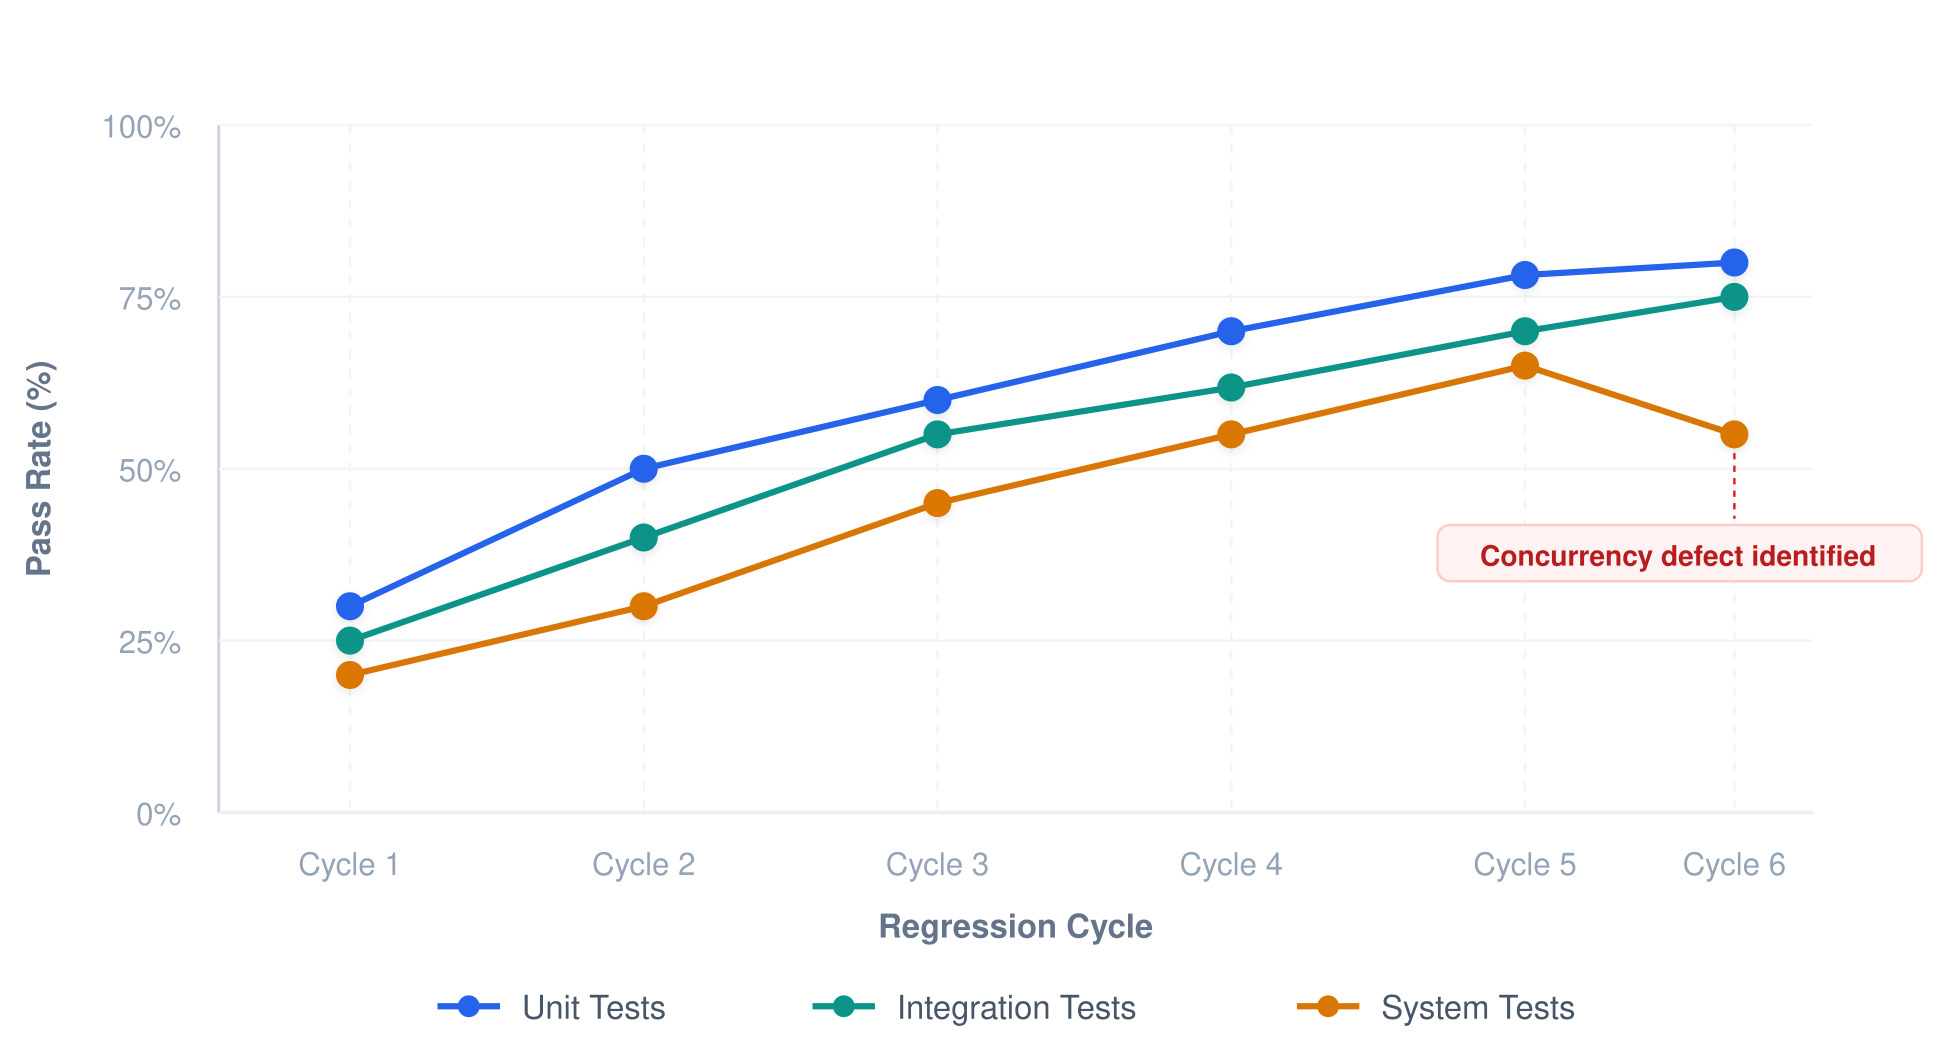
\includegraphics[width=0.82\textwidth]{regression_results_v2.jpg}
    \caption{Regression testing results}
    \label{fig:regression-results}
\end{figure}

\subsection{Summary of Testing}
% Writing good test cases / formatting / summary of results.

This test report has presented a structured and risk-aware testing strategy for the SPIO Competitor Benchmarking system across four levels: unit testing, integration testing, system testing, and user acceptance testing. To achieve broad but efficient coverage, 16 representative test cases were documented, with four at each level, using equivalence partitioning and boundary value analysis where appropriate. Each test case was defined with a clear oracle and expected outcome.

Overall, the testing results provide strong evidence that the system’s core functionality operates correctly across isolated units, integrated backend flows, end-to-end system behaviour, and user-facing tasks. The outcomes demonstrate that the implemented features function as intended and that the system performs reliably across the main scenarios considered within the scope of this project.

However, the results should be interpreted within the limits of the testing scope. As exhaustive testing is not feasible, the absence of further failures does not prove that the system is defect-free. Although targeted performance-related system testing was carried out, broader concurrent load and stress testing was outside the scope of this report. In addition, browser-based system tests were executed manually rather than through an automated end-to-end framework, and user acceptance testing was performed by the development team rather than an independent stakeholder group.

In summary, the testing process provided reasonable confidence in the correctness, stability, and usability of the current implementation across all four testing levels. Future testing should extend this work through broader concurrent-load testing, automated browser-based regression testing, and independent user acceptance testing with SPIO stakeholders in a production-like environment.

